\documentclass[1p]{elsarticle_modified}
%\bibliographystyle{elsarticle-num}

%\usepackage[colorlinks]{hyperref}
%\usepackage{abbrmath_seonhwa} %\Abb, \Ascr, \Acal ,\Abf, \Afrak
\usepackage{amsfonts}
\usepackage{amssymb}
\usepackage{amsmath}
\usepackage{amsthm}
\usepackage{scalefnt}
\usepackage{amsbsy}
\usepackage{kotex}
\usepackage{caption}
\usepackage{subfig}
\usepackage{color}
\usepackage{graphicx}
\usepackage{xcolor} %% white, black, red, green, blue, cyan, magenta, yellow
\usepackage{float}
\usepackage{setspace}
\usepackage{hyperref}

\usepackage{tikz}
\usetikzlibrary{arrows}

\usepackage{multirow}
\usepackage{array} % fixed length table
\usepackage{hhline}

%%%%%%%%%%%%%%%%%%%%%
\makeatletter
\renewcommand*\env@matrix[1][\arraystretch]{%
	\edef\arraystretch{#1}%
	\hskip -\arraycolsep
	\let\@ifnextchar\new@ifnextchar
	\array{*\c@MaxMatrixCols c}}
\makeatother %https://tex.stackexchange.com/questions/14071/how-can-i-increase-the-line-spacing-in-a-matrix
%%%%%%%%%%%%%%%

\usepackage[normalem]{ulem}

\newcommand{\msout}[1]{\ifmmode\text{\sout{\ensuremath{#1}}}\else\sout{#1}\fi}
%SOURCE: \msout is \stkout macro in https://tex.stackexchange.com/questions/20609/strikeout-in-math-mode

\newcommand{\cancel}[1]{
	\ifmmode
	{\color{red}\msout{#1}}
	\else
	{\color{red}\sout{#1}}
	\fi
}

\newcommand{\add}[1]{
	{\color{blue}\uwave{#1}}
}

\newcommand{\replace}[2]{
	\ifmmode
	{\color{red}\msout{#1}}{\color{blue}\uwave{#2}}
	\else
	{\color{red}\sout{#1}}{\color{blue}\uwave{#2}}
	\fi
}

\newcommand{\Sol}{\mathcal{S}} %segment
\newcommand{\D}{D} %diagram
\newcommand{\A}{\mathcal{A}} %arc


%%%%%%%%%%%%%%%%%%%%%%%%%%%%%5 test

\def\sl{\operatorname{\textup{SL}}(2,\Cbb)}
\def\psl{\operatorname{\textup{PSL}}(2,\Cbb)}
\def\quan{\mkern 1mu \triangleright \mkern 1mu}

\theoremstyle{definition}
\newtheorem{thm}{Theorem}[section]
\newtheorem{prop}[thm]{Proposition}
\newtheorem{lem}[thm]{Lemma}
\newtheorem{ques}[thm]{Question}
\newtheorem{cor}[thm]{Corollary}
\newtheorem{defn}[thm]{Definition}
\newtheorem{exam}[thm]{Example}
\newtheorem{rmk}[thm]{Remark}
\newtheorem{alg}[thm]{Algorithm}

\newcommand{\I}{\sqrt{-1}}
\begin{document}

%\begin{frontmatter}
%
%\title{Boundary parabolic representations of knots up to 8 crossings}
%
%%% Group authors per affiliation:
%\author{Yunhi Cho} 
%\address{Department of Mathematics, University of Seoul, Seoul, Korea}
%\ead{yhcho@uos.ac.kr}
%
%
%\author{Seonhwa Kim} %\fnref{s_kim}}
%\address{Center for Geometry and Physics, Institute for Basic Science, Pohang, 37673, Korea}
%\ead{ryeona17@ibs.re.kr}
%
%\author{Hyuk Kim}
%\address{Department of Mathematical Sciences, Seoul National University, Seoul 08826, Korea}
%\ead{hyukkim@snu.ac.kr}
%
%\author{Seokbeom Yoon}
%\address{Department of Mathematical Sciences, Seoul National University, Seoul, 08826,  Korea}
%\ead{sbyoon15@snu.ac.kr}
%
%\begin{abstract}
%We find all boundary parabolic representation of knots up to 8 crossings.
%
%\end{abstract}
%\begin{keyword}
%    \MSC[2010] 57M25 
%\end{keyword}
%
%\end{frontmatter}

%\linenumbers
%\tableofcontents
%
\newcommand\colored[1]{\textcolor{white}{\rule[-0.35ex]{0.8em}{1.4ex}}\kern-0.8em\color{red} #1}%
%\newcommand\colored[1]{\textcolor{white}{ #1}\kern-2.17ex	\textcolor{white}{ #1}\kern-1.81ex	\textcolor{white}{ #1}\kern-2.15ex\color{red}#1	}

{\Large $\underline{8_{17}~(K8a_{14})}$}

\setlength{\tabcolsep}{10pt}
\renewcommand{\arraystretch}{1.6}
\vspace{1cm}\begin{tabular}{m{100pt}>{\centering\arraybackslash}m{274pt}}
\multirow{5}{120pt}{
	\centering
	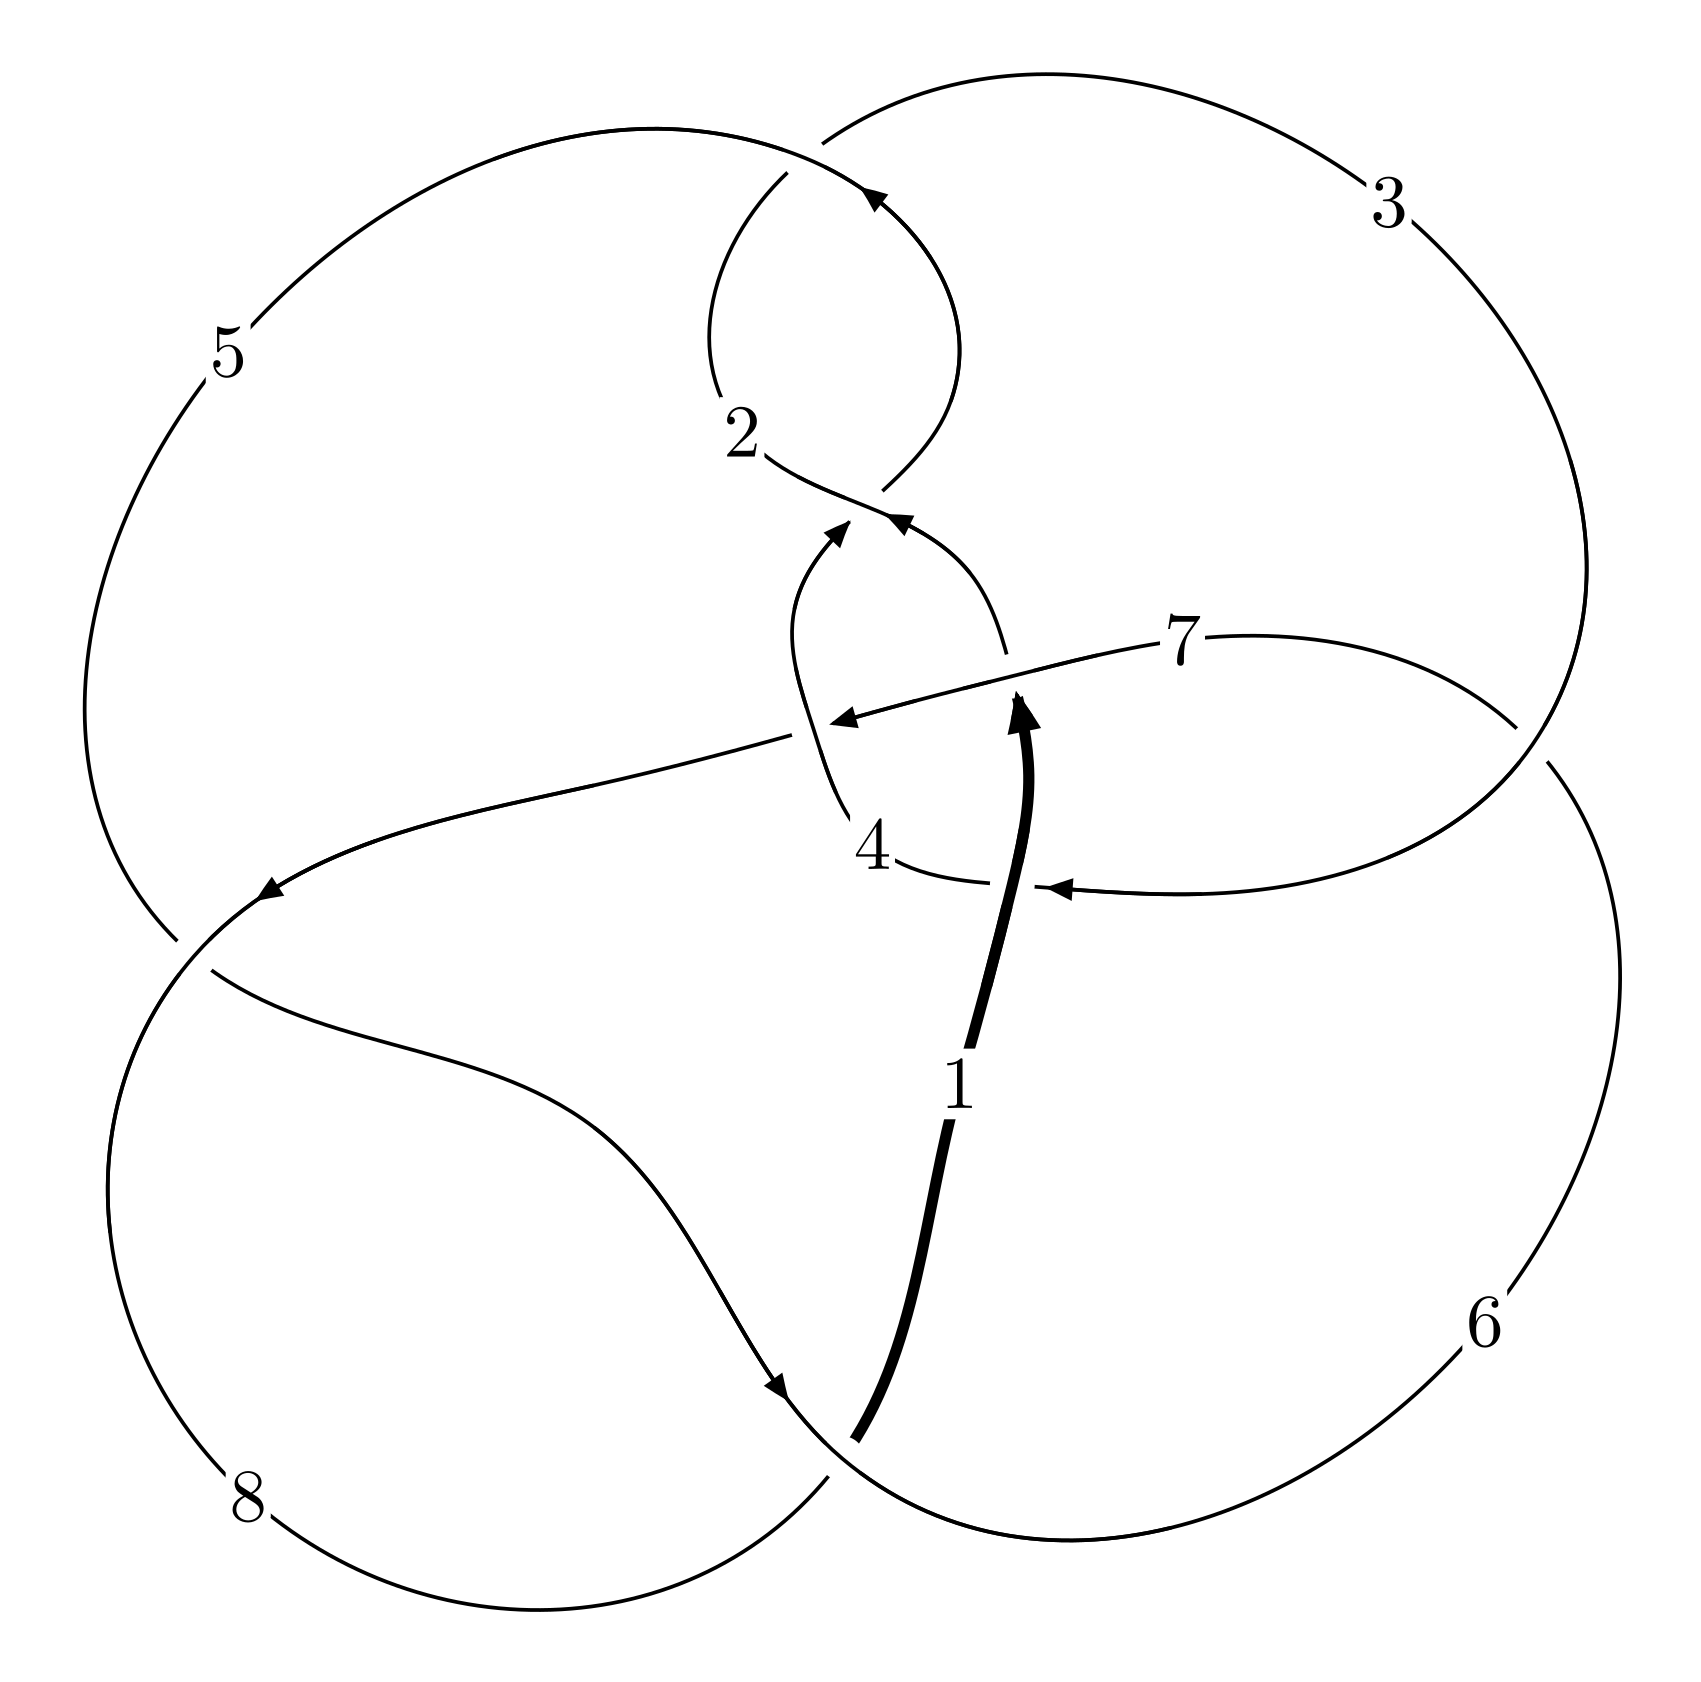
\includegraphics[width=112pt]{../../../GIT/diagram.site/Diagrams/png/31_8_17.png}\\
\ \ \ A knot diagram\footnotemark}&
\allowdisplaybreaks
\textbf{Linearized knot diagam} \\
\cline{2-2}
 &
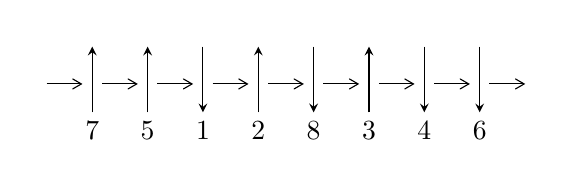
\begin{tikzpicture}[x=20pt, y=17pt]
	% nodes
	\node (C0) at (0, 0) {};
	\node (C1) at (1, 0) {};
	\node (C1U) at (1, +1) {};
	\node (C1D) at (1, -1) {7};

	\node (C2) at (2, 0) {};
	\node (C2U) at (2, +1) {};
	\node (C2D) at (2, -1) {5};

	\node (C3) at (3, 0) {};
	\node (C3U) at (3, +1) {};
	\node (C3D) at (3, -1) {1};

	\node (C4) at (4, 0) {};
	\node (C4U) at (4, +1) {};
	\node (C4D) at (4, -1) {2};

	\node (C5) at (5, 0) {};
	\node (C5U) at (5, +1) {};
	\node (C5D) at (5, -1) {8};

	\node (C6) at (6, 0) {};
	\node (C6U) at (6, +1) {};
	\node (C6D) at (6, -1) {3};

	\node (C7) at (7, 0) {};
	\node (C7U) at (7, +1) {};
	\node (C7D) at (7, -1) {4};

	\node (C8) at (8, 0) {};
	\node (C8U) at (8, +1) {};
	\node (C8D) at (8, -1) {6};
	\node (C9) at (9, 0) {};

	% arrows
	\draw[->,>={angle 60}]
	(C0) edge (C1) (C1) edge (C2) (C2) edge (C3) (C3) edge (C4) (C4) edge (C5) (C5) edge (C6) (C6) edge (C7) (C7) edge (C8) (C8) edge (C9) ;	\draw[->,>=stealth]
	(C1D) edge (C1U) (C2D) edge (C2U) (C3U) edge (C3D) (C4D) edge (C4U) (C5U) edge (C5D) (C6D) edge (C6U) (C7U) edge (C7D) (C8U) edge (C8D) ;
	\end{tikzpicture} \\
\hhline{~~} \\& 
\textbf{Solving Sequence} \\ \cline{2-2} 
 &
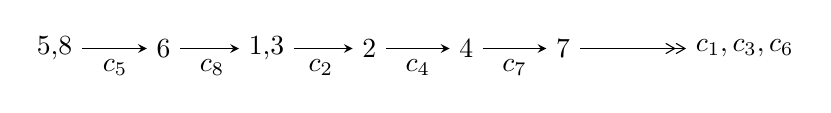
\begin{tikzpicture}[x=35pt, y=7pt]
	% node
	\node (A0) at (-1/8, 0) {5,8};
	\node (A1) at (1, 0) {6};
	\node (A2) at (33/16, 0) {1,3};
	\node (A3) at (25/8, 0) {2};
	\node (A4) at (33/8, 0) {4};
	\node (A5) at (41/8, 0) {7};
	\node (C1) at (1/2, -1) {$c_{5}$};
	\node (C2) at (3/2, -1) {$c_{8}$};
	\node (C3) at (21/8, -1) {$c_{2}$};
	\node (C4) at (29/8, -1) {$c_{4}$};
	\node (C5) at (37/8, -1) {$c_{7}$};
	\node (A6) at (7, 0) {$c_{1},c_{3},c_{6}$};

	% edge
	\draw[->,>=stealth]	
	(A0) edge (A1) (A1) edge (A2) (A2) edge (A3) (A3) edge (A4) (A4) edge (A5) ;
	\draw[->>,>={angle 60}]	
	(A5) edge (A6);
\end{tikzpicture} \\ 

\end{tabular} \\

\footnotetext{
The image of knot diagram is generated by the software ``\textbf{Draw programme}" developed by Andrew Bartholomew(\url{http://www.layer8.co.uk/maths/draw/index.htm\#Running-draw}), where we modified some parts for our purpose(\url{https://github.com/CATsTAILs/LinksPainter}).
}\phantom \\ \newline 
\centering \textbf{Ideals for irreducible components\footnotemark of $X_{\text{par}}$} 
 
\begin{align*}
I^u_{1}&=\langle 
-11044 u^{17}-26768 u^{16}+\cdots+654509 b-534698,\\
\phantom{I^u_{1}}&\phantom{= \langle  }-14404 u^{17}+515530 u^{16}+\cdots+654509 a-1200167,\;u^{18}+u^{17}+\cdots+3 u+1\rangle \\
\\
\end{align*}
\raggedright * 1 irreducible components of $\dim_{\mathbb{C}}=0$, with total 18 representations.\\
\footnotetext{All coefficients of polynomials are rational numbers. But the coefficients are sometimes approximated in decimal forms when there is not enough margin.}
\newpage
\renewcommand{\arraystretch}{1}
\centering \section*{I. $I^u_{1}= \langle -1.10\times10^{4} u^{17}-2.68\times10^{4} u^{16}+\cdots+6.55\times10^{5} b-5.35\times10^{5},\;-1.44\times10^{4} u^{17}+5.16\times10^{5} u^{16}+\cdots+6.55\times10^{5} a-1.20\times10^{6},\;u^{18}+u^{17}+\cdots+3 u+1 \rangle$}
\flushleft \textbf{(i) Arc colorings}\\
\begin{tabular}{m{7pt} m{180pt} m{7pt} m{180pt} }
\flushright $a_{5}=$&$\begin{pmatrix}1\\0\end{pmatrix}$ \\
\flushright $a_{8}=$&$\begin{pmatrix}0\\u\end{pmatrix}$ \\
\flushright $a_{6}=$&$\begin{pmatrix}1\\u^2\end{pmatrix}$ \\
\flushright $a_{1}=$&$\begin{pmatrix}- u\\- u^3+u\end{pmatrix}$ \\
\flushright $a_{3}=$&$\begin{pmatrix}0.0220073 u^{17}-0.787659 u^{16}+\cdots+2.49594 u+1.83369\\0.0168737 u^{17}+0.0408978 u^{16}+\cdots-0.737771 u+0.816945\end{pmatrix}$ \\
\flushright $a_{2}=$&$\begin{pmatrix}0.00513362 u^{17}-0.828557 u^{16}+\cdots+3.23371 u+1.01675\\0.0168737 u^{17}+0.0408978 u^{16}+\cdots-0.737771 u+0.816945\end{pmatrix}$ \\
\flushright $a_{4}=$&$\begin{pmatrix}-0.00366076 u^{17}-0.644874 u^{16}+\cdots+2.32739 u+1.74996\\-0.0674949 u^{17}-0.163591 u^{16}+\cdots-1.04891 u+0.732219\end{pmatrix}$ \\
\flushright $a_{7}=$&$\begin{pmatrix}-0.00251181 u^{17}-0.00174176 u^{16}+\cdots-1.88221 u-0.722479\\0.176743 u^{17}-0.811747 u^{16}+\cdots+3.33200 u+0.00509084\end{pmatrix}$\\&\end{tabular}
\flushleft \textbf{(ii) Obstruction class $= -1$}\\~\\
\flushleft \textbf{(iii) Cusp Shapes $= -\frac{2081176}{654509} u^{17}-\frac{1538700}{654509} u^{16}+\cdots+\frac{3609404}{654509} u+\frac{2997870}{654509}$}\\~\\
\newpage\renewcommand{\arraystretch}{1}
\flushleft \textbf{(iv) u-Polynomials at the component}\newline \\
\begin{tabular}{m{50pt}|m{274pt}}
Crossings & \hspace{64pt}u-Polynomials at each crossing \\
\hline $$\begin{aligned}c_{1}\end{aligned}$$&$\begin{aligned}
&u^{18}+3 u^{17}+\cdots+u+1
\end{aligned}$\\
\hline $$\begin{aligned}c_{2},c_{4}\end{aligned}$$&$\begin{aligned}
&u^{18}+u^{17}+\cdots+3 u+1
\end{aligned}$\\
\hline $$\begin{aligned}c_{3}\end{aligned}$$&$\begin{aligned}
&u^{18}-3 u^{17}+\cdots- u+1
\end{aligned}$\\
\hline $$\begin{aligned}c_{5},c_{8}\end{aligned}$$&$\begin{aligned}
&u^{18}- u^{17}+\cdots-3 u+1
\end{aligned}$\\
\hline $$\begin{aligned}c_{6}\end{aligned}$$&$\begin{aligned}
&u^{18}- u^{17}+\cdots+5 u+1
\end{aligned}$\\
\hline $$\begin{aligned}c_{7}\end{aligned}$$&$\begin{aligned}
&u^{18}+u^{17}+\cdots-5 u+1
\end{aligned}$\\
\hline
\end{tabular}\\~\\
\newpage\renewcommand{\arraystretch}{1}
\flushleft \textbf{(v) Riley Polynomials at the component}\newline \\
\begin{tabular}{m{50pt}|m{274pt}}
Crossings & \hspace{64pt}Riley Polynomials at each crossing \\
\hline $$\begin{aligned}c_{1},c_{3}\end{aligned}$$&$\begin{aligned}
&y^{18}-3 y^{17}+\cdots-3 y+1
\end{aligned}$\\
\hline $$\begin{aligned}c_{2},c_{4},c_{5}\\c_{8}\end{aligned}$$&$\begin{aligned}
&y^{18}-11 y^{17}+\cdots-3 y+1
\end{aligned}$\\
\hline $$\begin{aligned}c_{6},c_{7}\end{aligned}$$&$\begin{aligned}
&y^{18}+13 y^{17}+\cdots-3 y+1
\end{aligned}$\\
\hline
\end{tabular}\\~\\
\newpage\flushleft \textbf{(vi) Complex Volumes and Cusp Shapes}
$$\begin{array}{c|c|c}  
\text{Solutions to }I^u_{1}& \I (\text{vol} + \sqrt{-1}CS) & \text{Cusp shape}\\
 \hline 
\begin{aligned}
u &= -0.912810 + 0.341070 I \\
a &= \phantom{-}0.50288 + 1.83925 I \\
b &= \phantom{-}1.168300 + 0.720176 I\end{aligned}
 & \phantom{-}1.46999 + 3.11720 I & \phantom{-}3.21326 - 6.66243 I \\ \hline\begin{aligned}
u &= -0.912810 - 0.341070 I \\
a &= \phantom{-}0.50288 - 1.83925 I \\
b &= \phantom{-}1.168300 - 0.720176 I\end{aligned}
 & \phantom{-}1.46999 - 3.11720 I & \phantom{-}3.21326 + 6.66243 I \\ \hline\begin{aligned}
u &= \phantom{-}0.950168 + 0.130449 I \\
a &= \phantom{-}0.05948 - 3.09238 I \\
b &= \phantom{-}0.950168 - 0.130449 I\end{aligned}
 & \phantom{-0.000000 } -0.520528 I & \phantom{-0.000000 } 0. - 13.01684 I \\ \hline\begin{aligned}
u &= \phantom{-}0.950168 - 0.130449 I \\
a &= \phantom{-}0.05948 + 3.09238 I \\
b &= \phantom{-}0.950168 + 0.130449 I\end{aligned}
 & \phantom{-0.000000 -}0.520528 I & \phantom{-0.000000 -}0. + 13.01684 I \\ \hline\begin{aligned}
u &= -0.167072 + 1.125400 I \\
a &= \phantom{-}0.300048 + 0.121690 I \\
b &= -1.190060 + 0.368733 I\end{aligned}
 & \phantom{-}3.57267 - 4.95181 I & \phantom{-}3.31278 + 5.61624 I \\ \hline\begin{aligned}
u &= -0.167072 - 1.125400 I \\
a &= \phantom{-}0.300048 - 0.121690 I \\
b &= -1.190060 - 0.368733 I\end{aligned}
 & \phantom{-}3.57267 + 4.95181 I & \phantom{-}3.31278 - 5.61624 I \\ \hline\begin{aligned}
u &= -1.190060 + 0.368733 I \\
a &= -0.385891 + 1.324270 I \\
b &= -0.167072 + 1.125400 I\end{aligned}
 & -3.57267 + 4.95181 I & -3.31278 - 5.61624 I \\ \hline\begin{aligned}
u &= -1.190060 - 0.368733 I \\
a &= -0.385891 - 1.324270 I \\
b &= -0.167072 - 1.125400 I\end{aligned}
 & -3.57267 - 4.95181 I & -3.31278 + 5.61624 I \\ \hline\begin{aligned}
u &= \phantom{-}1.342100 + 0.135496 I \\
a &= -0.083889 - 0.268734 I \\
b &= -0.470709 - 0.243089 I\end{aligned}
 & -2.59619 - 0.05903 I & -5.04488 - 1.45254 I \\ \hline\begin{aligned}
u &= \phantom{-}1.342100 - 0.135496 I \\
a &= -0.083889 + 0.268734 I \\
b &= -0.470709 + 0.243089 I\end{aligned}
 & -2.59619 + 0.05903 I & -5.04488 + 1.45254 I\\
 \hline 
 \end{array}$$\newpage$$\begin{array}{c|c|c}  
\text{Solutions to }I^u_{1}& \I (\text{vol} + \sqrt{-1}CS) & \text{Cusp shape}\\
 \hline 
\begin{aligned}
u &= \phantom{-}1.168300 + 0.720176 I \\
a &= \phantom{-}0.337342 + 0.860665 I \\
b &= -0.912810 + 0.341070 I\end{aligned}
 & -1.46999 - 3.11720 I & -3.21326 + 6.66243 I \\ \hline\begin{aligned}
u &= \phantom{-}1.168300 - 0.720176 I \\
a &= \phantom{-}0.337342 - 0.860665 I \\
b &= -0.912810 - 0.341070 I\end{aligned}
 & -1.46999 + 3.11720 I & -3.21326 - 6.66243 I \\ \hline\begin{aligned}
u &= -1.30098 + 0.59320 I \\
a &= -0.11190 - 1.47782 I \\
b &= -1.30098 - 0.59320 I\end{aligned}
 & \phantom{-0.000000 -}10.9859 I & \phantom{-0.000000 } 0. - 7.09338 I \\ \hline\begin{aligned}
u &= -1.30098 - 0.59320 I \\
a &= -0.11190 + 1.47782 I \\
b &= -1.30098 + 0.59320 I\end{aligned}
 & \phantom{-0.000000 } -10.9859 I & \phantom{-0.000000 -}0. + 7.09338 I \\ \hline\begin{aligned}
u &= \phantom{-}0.081063 + 0.532154 I \\
a &= \phantom{-}0.989810 - 0.121474 I \\
b &= \phantom{-}0.081063 - 0.532154 I\end{aligned}
 & \phantom{-0.000000 } -1.47534 I & \phantom{-0.000000 -}0. + 4.20317 I \\ \hline\begin{aligned}
u &= \phantom{-}0.081063 - 0.532154 I \\
a &= \phantom{-}0.989810 + 0.121474 I \\
b &= \phantom{-}0.081063 + 0.532154 I\end{aligned}
 & \phantom{-0.000000 -}1.47534 I & \phantom{-0.000000 } 0. - 4.20317 I \\ \hline\begin{aligned}
u &= -0.470709 + 0.243089 I \\
a &= \phantom{-}0.892107 + 0.422485 I \\
b &= \phantom{-}1.342100 - 0.135496 I\end{aligned}
 & \phantom{-}2.59619 - 0.05903 I & \phantom{-}5.04488 - 1.45254 I \\ \hline\begin{aligned}
u &= -0.470709 - 0.243089 I \\
a &= \phantom{-}0.892107 - 0.422485 I \\
b &= \phantom{-}1.342100 + 0.135496 I\end{aligned}
 & \phantom{-}2.59619 + 0.05903 I & \phantom{-}5.04488 + 1.45254 I\\
 \hline 
 \end{array}$$\newpage
\newpage\renewcommand{\arraystretch}{1}
\centering \section*{ II. u-Polynomials}
\begin{tabular}{m{50pt}|m{274pt}}
Crossings & \hspace{64pt}u-Polynomials at each crossing \\
\hline $$\begin{aligned}c_{1}\end{aligned}$$&$\begin{aligned}
&u^{18}+3 u^{17}+\cdots+u+1
\end{aligned}$\\
\hline $$\begin{aligned}c_{2},c_{4}\end{aligned}$$&$\begin{aligned}
&u^{18}+u^{17}+\cdots+3 u+1
\end{aligned}$\\
\hline $$\begin{aligned}c_{3}\end{aligned}$$&$\begin{aligned}
&u^{18}-3 u^{17}+\cdots- u+1
\end{aligned}$\\
\hline $$\begin{aligned}c_{5},c_{8}\end{aligned}$$&$\begin{aligned}
&u^{18}- u^{17}+\cdots-3 u+1
\end{aligned}$\\
\hline $$\begin{aligned}c_{6}\end{aligned}$$&$\begin{aligned}
&u^{18}- u^{17}+\cdots+5 u+1
\end{aligned}$\\
\hline $$\begin{aligned}c_{7}\end{aligned}$$&$\begin{aligned}
&u^{18}+u^{17}+\cdots-5 u+1
\end{aligned}$\\
\hline
\end{tabular}\newpage\renewcommand{\arraystretch}{1}
\centering \section*{ III. Riley Polynomials}
\begin{tabular}{m{50pt}|m{274pt}}
Crossings & \hspace{64pt}Riley Polynomials at each crossing \\
\hline $$\begin{aligned}c_{1},c_{3}\end{aligned}$$&$\begin{aligned}
&y^{18}-3 y^{17}+\cdots-3 y+1
\end{aligned}$\\
\hline $$\begin{aligned}c_{2},c_{4},c_{5}\\c_{8}\end{aligned}$$&$\begin{aligned}
&y^{18}-11 y^{17}+\cdots-3 y+1
\end{aligned}$\\
\hline $$\begin{aligned}c_{6},c_{7}\end{aligned}$$&$\begin{aligned}
&y^{18}+13 y^{17}+\cdots-3 y+1
\end{aligned}$\\
\hline
\end{tabular}
\vskip 2pc
\end{document}